\chapter{The \CMS experiment}
\label{chap:detector}

\section{The \LHC}
\label{sec:theLHC}

The Large Hadron Collider (LHC) \cite{theLHC} is synchrotron acceralator
with a $27 km$ circumference designed to
collide beams of protons at centre of mass energies as high as $14~\TeV$. It is
hosted in the former tunnel of the Large Electron Positron (LEP) \cite{LEP:1983aa} experiment on the French-Swiss border
near Geneva and operated by the European Organisation for Nuclear Research
(CERN). As well as proton-proton collisions, the LHC also accelerates beams of
lead ions to produce both lead-lead (PbPb) and proton-lead (pPb) collisions.

The protons originate from hydrogen gas, the atoms of which are stripped of
their electrons using an electric field. The protons are then accelerated to an
energy of $50~\MeV$ in the Linac 2 accelerator. Proton bunches are formed inside
the \ac{PSB}, increasing the energy to $1.4~\GeV$. The \ac{PS} creates proton
beams from the bunches, increasing the energy to $26~\GeV$. Further acceleration
in the \ac{SPS} raises the beam energy to $450~\GeV$ before being injected into
the LHC. The LHC contains two beams circulating in opposite directions. The
design operation conditions consist of each beam containing up to 2800 bunches
spaced $25~\ns$ apart and made up of $\mathcal{O}(10^{11})$ protons each. 
Approximately 1200 superconducting dipole magnets keep the beams circulating
before collisions. The beams collide at four points around the LHC where they
are recorded by four detectors: ALICE \cite{Aamodt:2008zz}, ATLAS
\cite{Aad:2008zzm}, CMS \cite{Chatrchyan:2008aa} and LHCb \cite{Alves:2008zz}. A
schematic of the LHC ring and the detectors is shown in figure
\ref{fig:LHCschematic}.

\begin{figure}[htbp]
   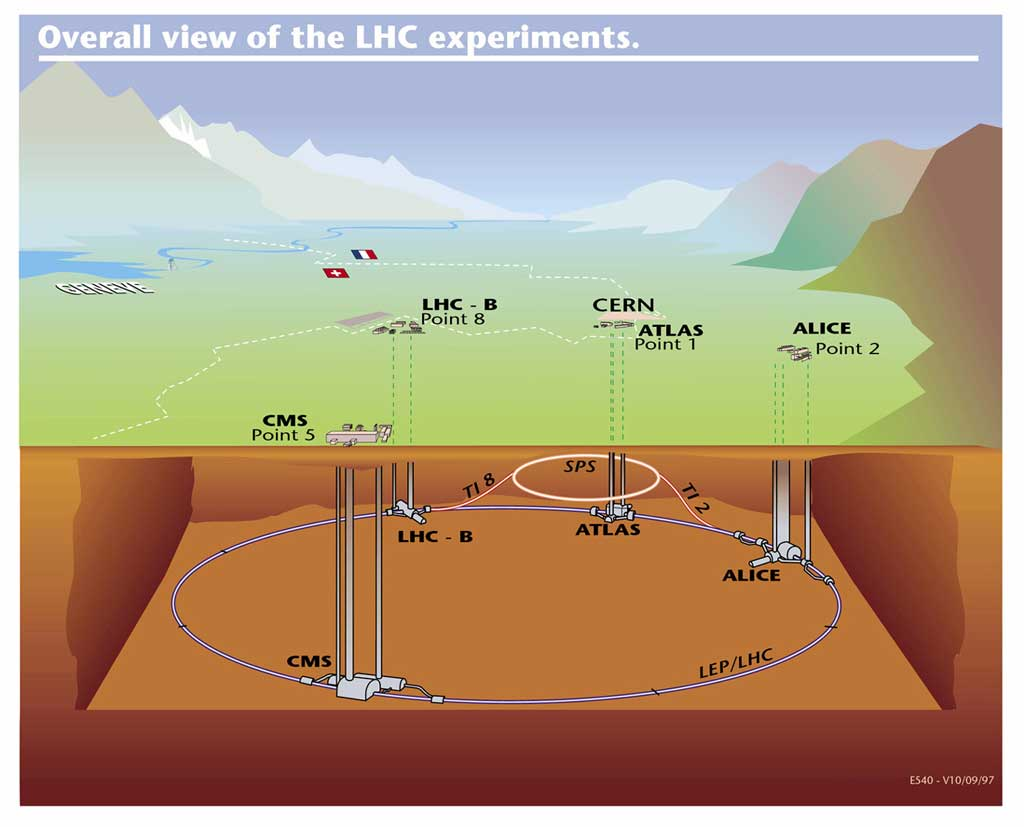
\includegraphics[width=0.6\textwidth]{plots/detector/LHC_layout_sch.jpg}
\caption{Schematic of the LHC accelerator, showing the positions of the four
large detectors.}
\label{fig:LHCschematic}
\end{figure}

The LHC was designed to study physics at the $\TeV$ scale. One of the major
goals of the ATLAS and CMS detectors is to understand the mechanism behind
electroweak symmetry breaking, and search for the Higgs boson predicted by this
mechanism in the \ac{SM}. The detectors are also used in searches for \ac{BSM}
physics, with the huge acceleration power of the LHC allowing studies of 
interactions at higher energies than have ever been possible before. 

Many such processes occur only rarely amongst other possible interactions from known
\ac{SM} processes. Figure \ref{fig:LHCcrosssections} shows the cross-sections of
such processes compared with the total proton-proton cross-section. It can be
seen that Higgs boson production has a cross-section some $10^{-9}$ times
smaller than the total proton-proton cross-section. 
As such, it is necessary to collect large numbers of
collisions to ensure sufficient numbers of events containing such rare
processes. Hence the LHC operates at a high instantaneous luminosity of up to
$10^{34}\,\lumiunits$, where luminosity is defined as:

\begin{equation}
L=\frac{N_{b}^{2}n_{b}f_{\text{rev}}\gamma}{4\pi\epsilon_{n}\beta^{*}}F,
\end{equation}

where $N_{b}$ is the number of protons in the bunch, $n_{b}$ is the number of
bunches, $f_\text{rev}$ is the revolution frequency, $\gamma$ is the Lorentz
factor, $\epsilon_{n}$ is the normalised emittance, $\beta^{*}$ is the beta
function at the collision point and $F$ is a reduction factor due to the
crossing angle.

\begin{figure}[htbp]
   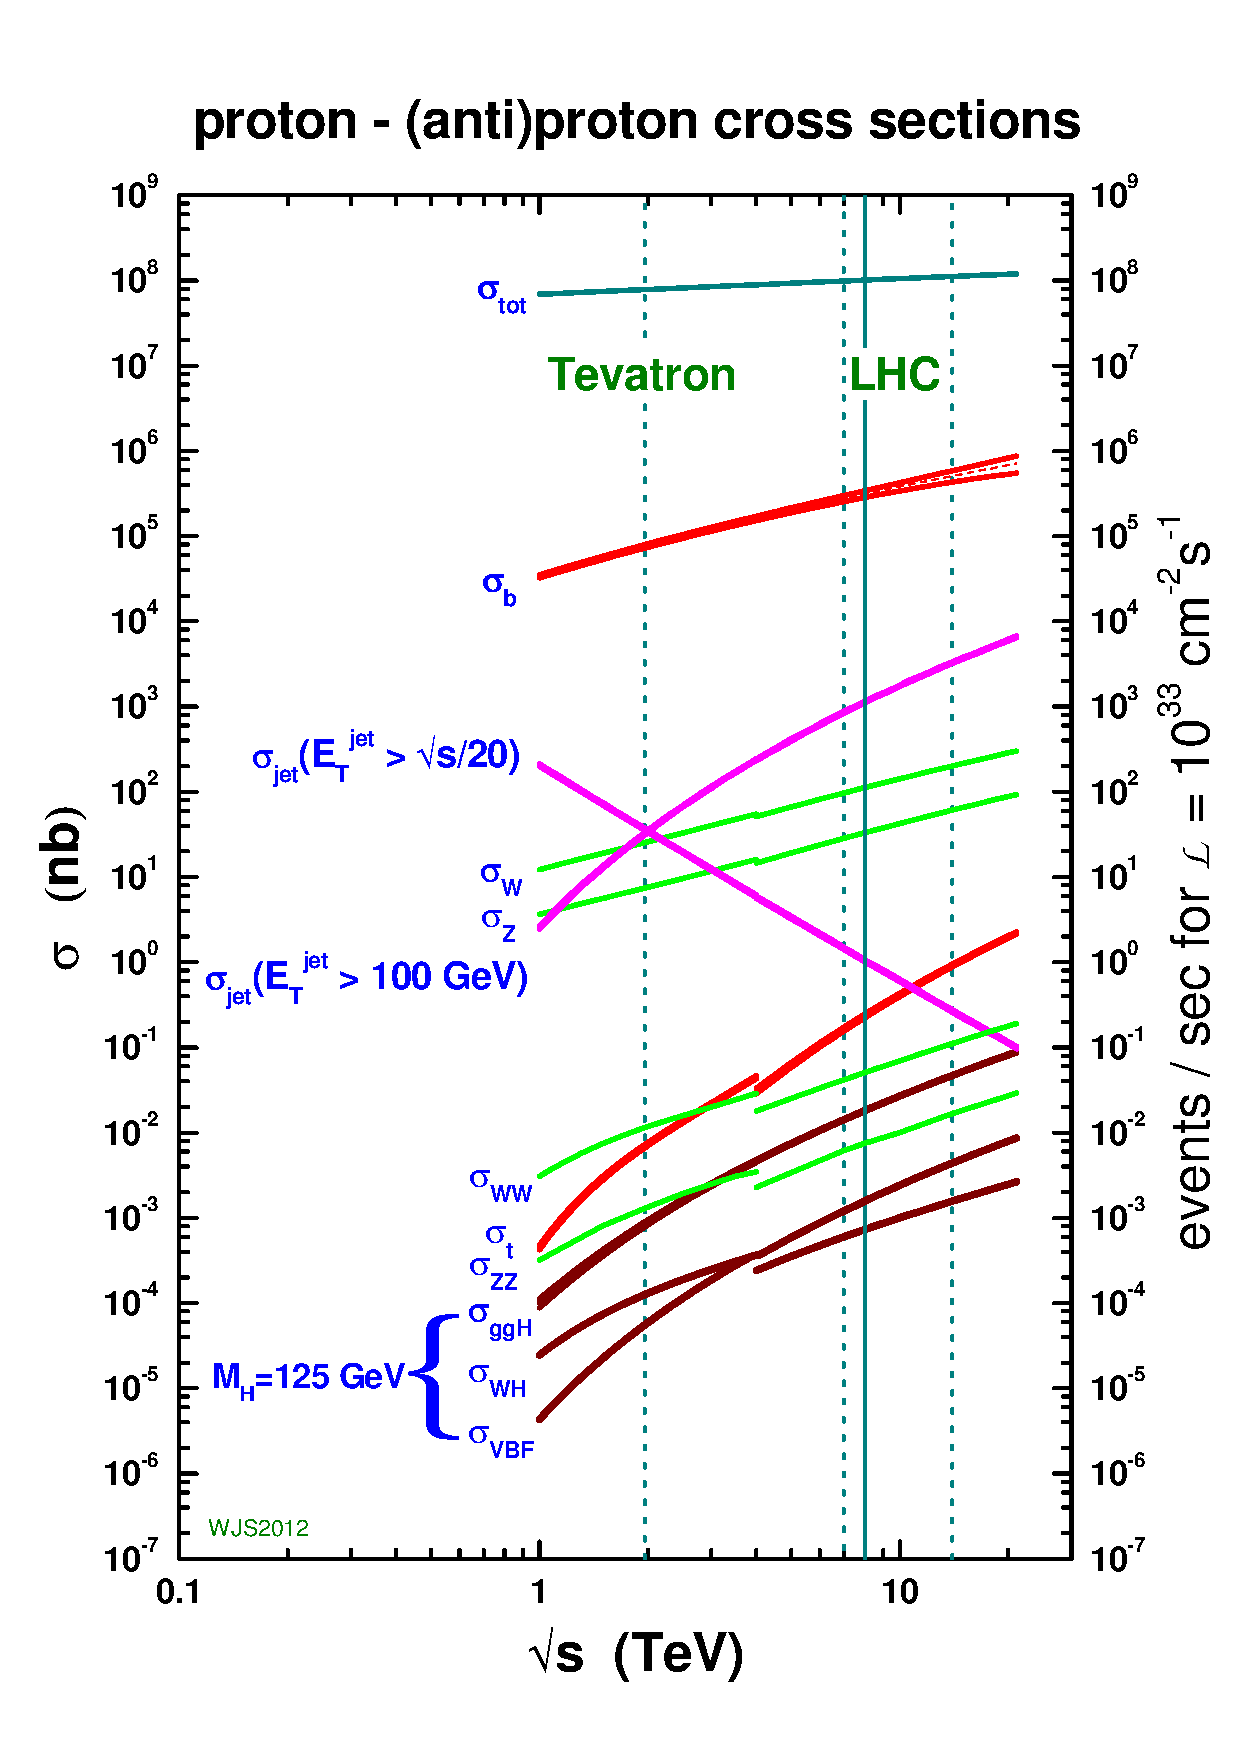
\includegraphics[width=0.6\textwidth]{plots/detector/crosssections2012_v5.pdf}
\caption{Cross sections for several processes in proton-proton or proton-anti
proton collisions, dependent on centre of mass energy. Energies of the LHC at
different points in running history are highlighted, as is the energy of the
Tevatron. It can be seen that even with the high energies of the LHC, the
cross-section for Higgs boson production is several orders of magnitude smaller than
the total cross-section \cite{stirling:xsecs}.}
\label{fig:LHCcrosssections}
\end{figure}

The \ac{LHC} began its first major physics run in May 2010 with a centre of mass
energy of $\sqrt{s} = 7~\TeV$ and produced $44.2~\invpb$ in its first run
before stopping for the winter break. It then continued at $\sqrt{s} = 7~\TeV$
producing an integrated luminosity of $5.6~\invfb$, before increasing to
$\sqrt{s} = 8~\TeV$ for the 2012 run, where it collected $23.3~\invfb$.
During this time the LHC operated with a bunch spacing of $50~\ns$. It
was after the 2011 run and $\approx6~\invfb$ of the 2012 run that the
observation of a boson consistent with the Higgs boson of the \ac{SM} was
announced in July 2012. Figure~\ref{fig:detlumi} shows the summary of the
integrated luminosity collected by the CMS detector during run 1 of the LHC,
which concluded in early 2013. Not all luminosity delivered by the LHC is
certified for use in physics analyses - only those events where it is known that
the whole CMS detector was operating successfully, and so this reduced the
usable dataset to $5.1\,\invfb$ in 2011 and $19.7\,\invfb$ in 2012.

\begin{figure}[htbp]
   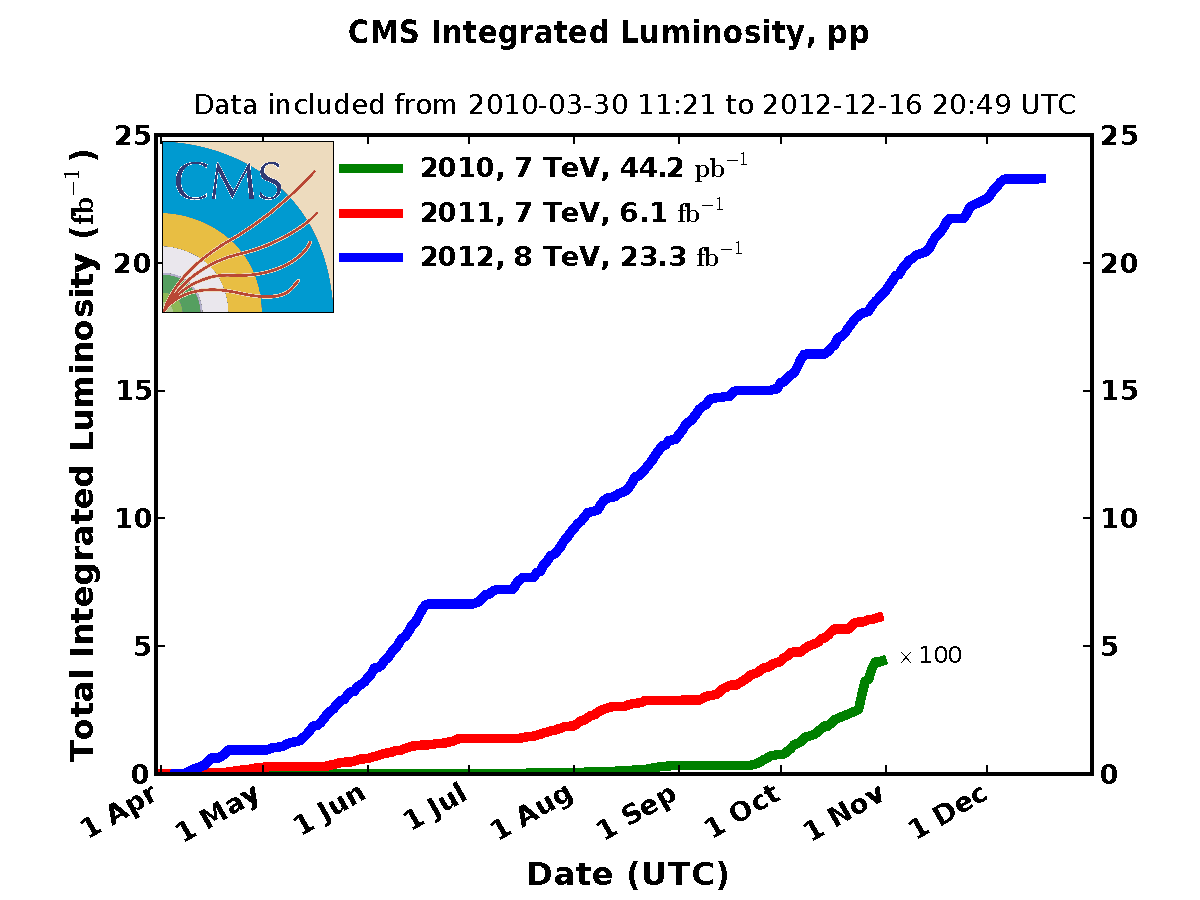
\includegraphics[width=0.7\textwidth]{plots/detector/int_lumi_cumulative_pp_2.pdf}
\caption{Illustration of the total integrated luminosty collected by CMS during run 1 of the
LHC, split into the 3 years of running \cite{cmslumitwiki}.}
\label{fig:detlumi}
\end{figure}

Since the LHC operates at such high luminosity, the probability of multiple
proton-proton collisions ocurring in each bunch crossing is very high. Figure
~\ref{fig:reco-nint} shows the number of interactions per bunch crossing in the
2012 dataset, where the average number was 21. The number for 2011 was slightly
lower due to the lower instantaneous luminosity at 9. 
These additional collisions on top of the interesting
underlying process in an event are referred to as pileup.

\begin{figure}[htbp]
   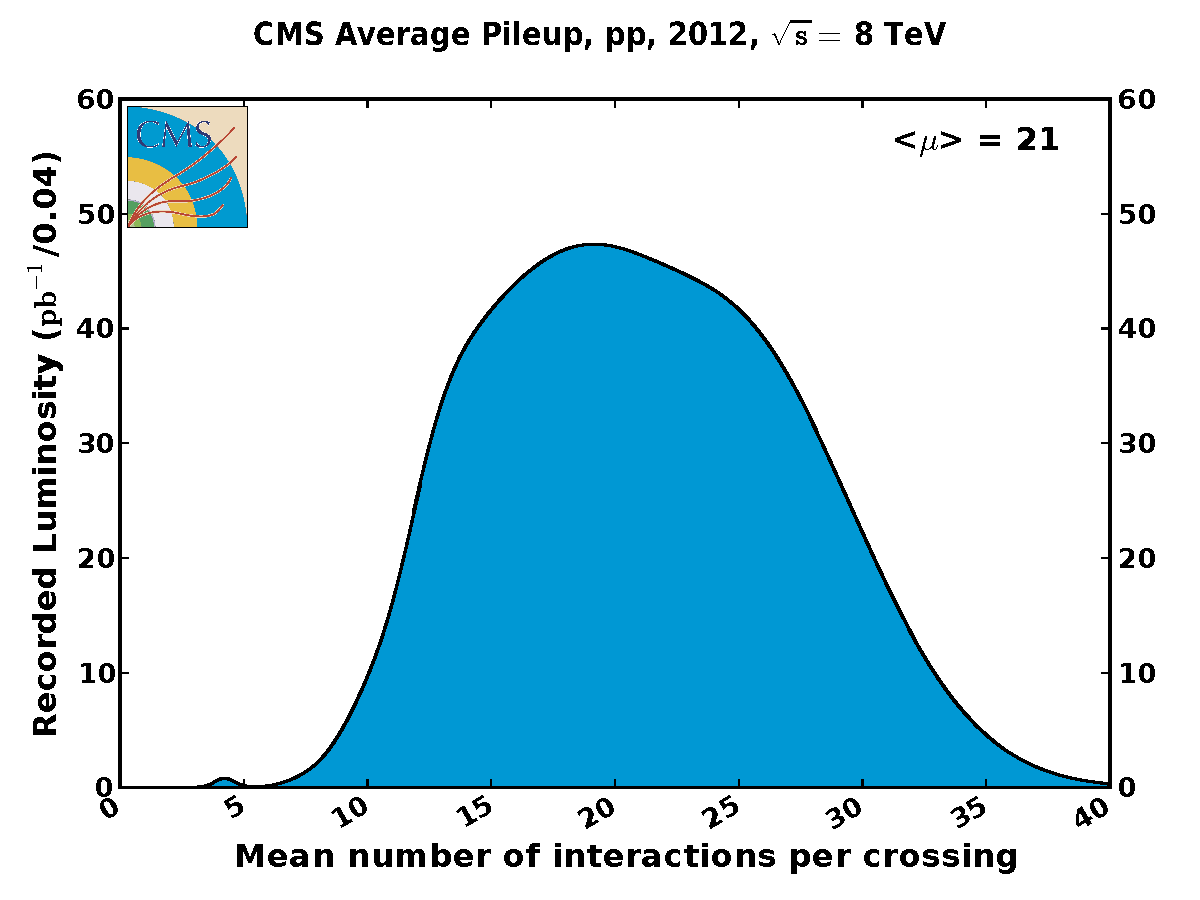
\includegraphics[width=0.7\textwidth]{plots/detector/pileup_pp_2012-2.pdf}
\caption{Distribution of number of pileup events per bunch crossing in 2012 data \cite{cmslumitwiki}.}
\label{fig:detlumi}
\end{figure}

\section{The \CMS experiment}
\label{sec:CMSInDetail}

The CMS detector is a general purpose detector designed to search for the
\ac{SM} Higgs and new physics. As discussed in section~\ref{sec:smhiggs}, the
mass of the Higgs boson is not directly predicted by the \ac{SM}, and hence it
was important that CMS be able to achieve sensitivity to the \ac{SM} Higgs for a
wide range of possible masses. As shown in figure~\ref{fig:SMbrs}, at different
Higgs masses the branching ratios of the Higgs boson to different final states
vary a lot, and as such CMS must be able to detect the particles from all
possible decay channels. To achieve this, CMS is a hermetic detector featuring
a layered system of different subdetectors, each of importance to the detection
of different particles. A slice of the CMS detector can be seen in
figure~\ref{fig:CMSslice}.

\begin{figure}[htbp]
   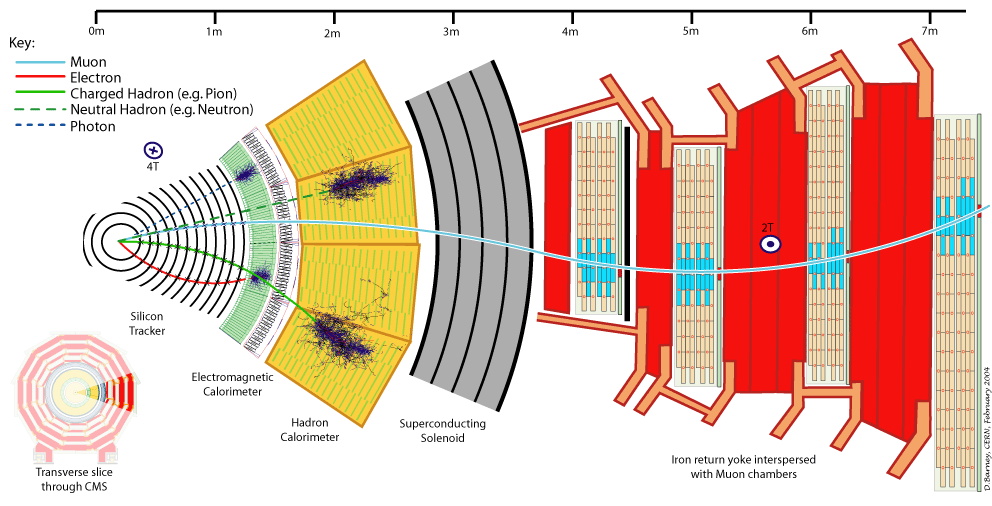
\includegraphics[width=0.9\textwidth]{plots/detector/CMS_Slice.png}
\caption{A slice of the CMS detector, indicating the various subdetectors. The
paths taken by different types of particles travelling through the detector are
indicated.}
\label{fig:CMSslice}
\end{figure}

The first layer is the tracker, which records the tracks of charged particles,
from which can be extracted the particles momentum and the location of the
vertex it originated from. This is followed by the \ac{ECAL} which measures
energy desposited in electromagnetic showers from electrons or photons. The
\ac{HCAL} does a similar job for the hadronic activity, by providing energy
measurements of collections of hadrons, known as jets, which deposit energy
through nuclear interactions. The \ac{HCAL} is a sampling calorimeter, meaning
that the active material is sandwiched between dense absorbing material to
increase the depth of the calorimeter to around 11 radiation lengths. The
\ac{HCAL} coverage is increased in the forward regions by the addition of 
the \ac{HF} calorimeter. The tracker and calorimeters are encased within a 3.8T axial magnetic
field provided by a superconducting magnet which forms the next layer. This
magnet field provides the mechanism for directing the charged particle tracks in
a curve such that their momentum can be measured by the size of the curve and
their charge by the direction. The
outermost layers form the muon detector systems, interspersed with iron plates
of the return yoke of the magnet. Muons desposit little energy
through the detector and often travel through to the surrounding cavern. The
whole CMS detector is $22~\metre$ long and $15~\metre$ in diameter
\cite{Chatrchyan:2008aa}.

CMS uses a right handed cartesian coordinate system. The
origin is placed at the interaction point with the $z$ axis collinear with the
beam. Then the $x$ axis is chosen to point towards the centre of the LHC ring
and forms a plane with $y$, the remaining transverse coordinate perpendicular to
$x$ and $z$. The angle $\phi$ is the azimuthal angle with respect to the $x$
axis and $\theta$ is the polar angle in the $x-y$ plane. Another coordinate
often used is pseudorapidity, defined as:
\begin{equation}
\eta = - \ln[\tan(\theta/2)]. 
\end{equation}

Distance in the $\eta$-$\phi$ plane is given by $\Delta R =
\sqrt{\Delta\phi^{2} + \Delta\eta^{2}}$.
Another important quantity relating to the measurement of collisions is the
projection of the momentum of a particle onto the transverse plane: $\pt =
\sqrt{p_{x}^{2} + p_{y}^{2}}$. The corresponding transverse energy is referred
to as $E_{\text T}$. Hard collisions generally produce particles with
high $\pt$.

\subsection{Tracker}
\label{sec:tracker}

The CMS tracker is designed to reconstruct charged particles close to the
interaction point \cite{Chatrchyan:2008aa}. The magnetic field in combination with the tracker allows
measurement of the particles momenta and charges. This requires a high level of
granularity to make precise measurements of positions of particles and hence to
locate the vertex from which they originate. Due to the design bunch spacing of
$25ns$ of the LHC the rate of collision is extremely high, and so the tracker is
required to be fast response and radiation hard. This motivates the use of a
silicon based tracking system.

The tracker is composed of layers of silicon pixel and strip detectors covering
the pseudorapidity range $|\eta| < 2.5$. The pixel detector consists of 66
million individual silicon pixels, each $100~\micron \times 150~\micron$
in size, forming three layers in the barrel region and two in each endcap. The
resolution of the pixel detector is $15$--$20\micron$ in the $r$-$\phi$ plane
and the $z$ direction, allowing a three-dimensional vertex reconstruction.
Surrounding the pixel detector are layers of strip detectors. These consist of
four cyclindrical layers which extend to $r=55\,\cm$ referred to as the
\ac{TIB}, and three disks in each endcap refered to as the \ac{TID}. Each strip
is $10$--$20\,\cm$ long and $80$--$180\,\micron$ wide. Surrounding the \ac{TIB}
and \ac{TID} is the \ac{TOB}, which which extends to $r=116\,\cm$ and
$z\pm118\,\cm$ and contains six barrel layers. The \ac{TEC} is comprised of nine
disks covering the endcaps. This geometry is shown in figure
\ref{fig:trackerlayout}.

\begin{figure}[htbp]
   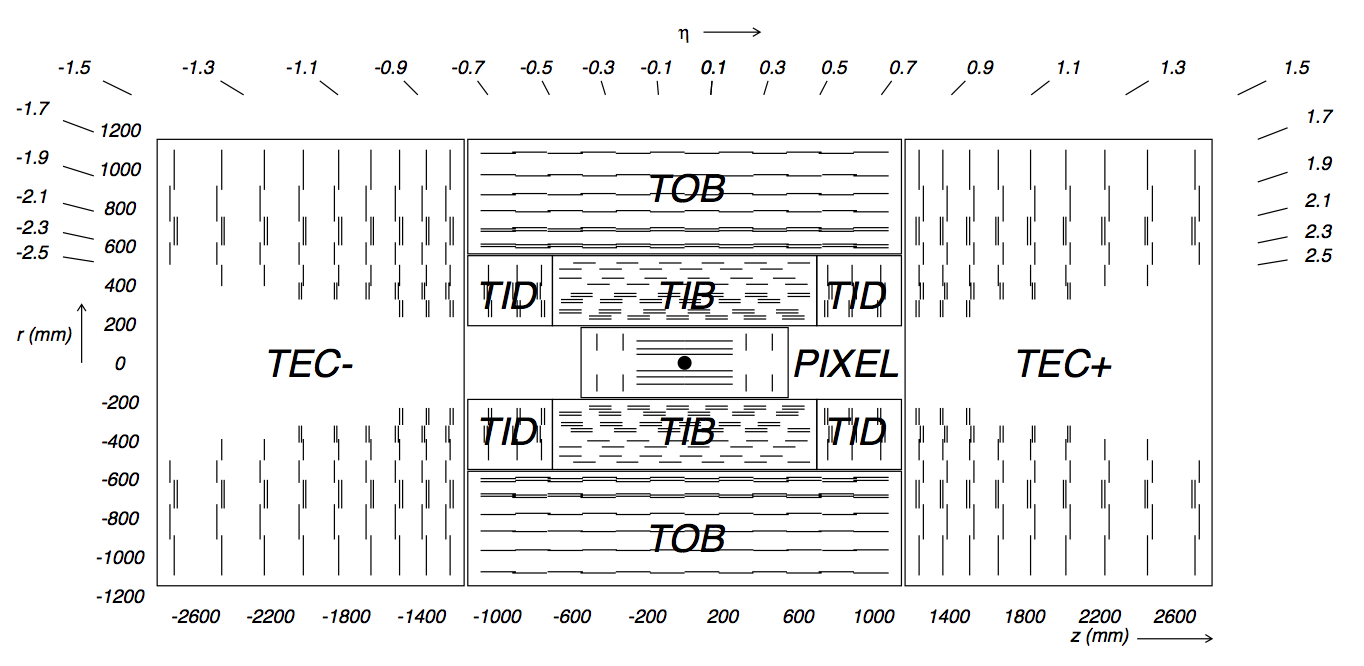
\includegraphics[width=0.9\textwidth]{plots/detector/tracker_layout.png}
\caption{Cross-section of the CMS tracking system, indicating the pixel and
strip detectors and their positions inside the detector \cite{Chatrchyan:2008aa}.}
\label{fig:trackerlayout}
\end{figure}

Tracks are reconstructed using multiple precise measurements throughout the
tracking system. The reconstruction is seeded by triplets of hits in the inner
tracking layers. The trajory of this seed is extrapolated to the outer tracking
layers using the Kalman filter method \cite{}. The hits found in each layer
which are compatible are added to the trajectory and its uncertainties are
updated until no more compatible hits are found. The use of the tracks to
reconstruct the \ac{PV} is discussed further in section \ref{sec:vertex}.

\subsection{Electromagnetic calorimeter}
\label{sec:ecal}

The \ac{ECAL} is constructed from high density lead tungstate
($\mathrm{PbWO_{4}}$) crystals which form a barrel section (EB) 
and two endcaps (EE) outside the tracker. $\mathrm{PbWO_{4}}$ was chosen for its
radiation hardness, short radiation length ($0.89~\cm$) and small Moli\`ere
radius ($2.2\,\cm$), meaning that almost the entire photon or electron energy
can be deposited in the \ac{ECAL}. High energy electrons or photons
entering a crystal initiate an electromagnetic shower, which produces a cascade
of low energy electrons and photons which undergo bremsstrahlung and pair
production respectively. The shower will continue until energy falls below pair
production threshold and ionisation begins to dominate for electrons. 
The depth of each crystal is equivalent to 25.8 radiation lengths, and
thus electrons and photons deposit most of their energy within the crystals.
The atoms in the $\mathrm{PbWO_{4}}$ de-excite by producing scintillation light that is read by
photodetectors. The decay time of the scintillation light is short, such that
about 80\% is emitted before the next bunch crossing (within $25~\ns$). This
results in a calorimter with excellent energy resoltuion, granularity and timing
precision.

Figure \ref{fig:ecal} shows the layout of the \ac{ECAL}. The EB covers the
pseudorapidity range $|\eta|<1.479$. The crystals are arranged in 36 modules such
that the gap between modules are offset by $3\circ$ with respect to the axis
from the detector origin to avoid particles travelling along the gaps between
crystals. In
the endcaps the crystals are arranged in an $x$-$y$ grid each with an area of
28.6$\,\times\,$28.6 $\mathrm{mm^{2}}$. Two lead plates and two silicon strip
layers mounted before the EE form the pre-shower detectors (PS). These correspond to about
$3$ radiation lengths of absorber material and are designed to initiate
showering and provide sufficient resolution to distinguish single photons from
the pairs produced in neutral pion decays. Uninstrumented regions exist
between the EB and EE, $1.442 < |\eta| < 1.566$, through which cables pass. It
is not possible to provide good measurement of electrons and photons traversing
this region. Overall the \ac{ECAL} covers a pseudorapidity range of $|\eta|<3$.

\begin{figure}[htbp]
   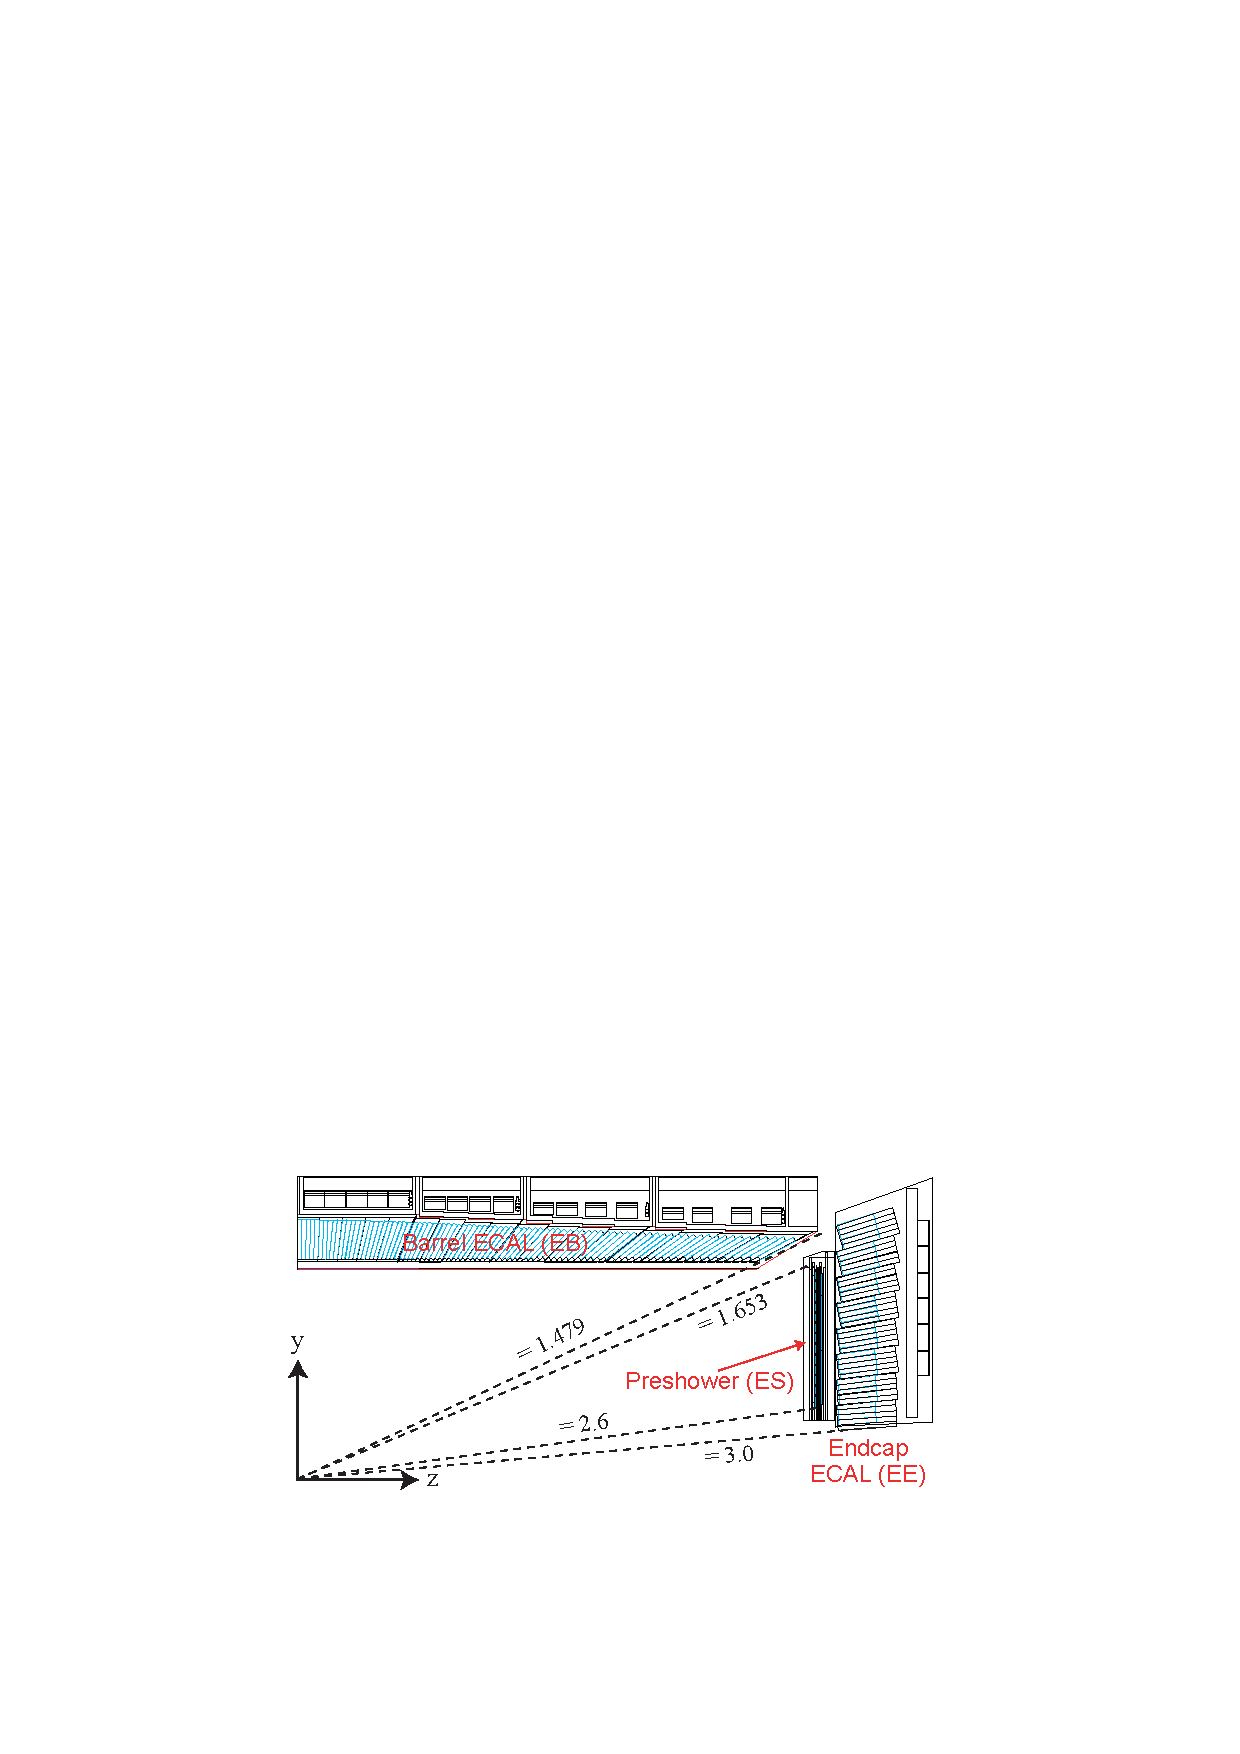
\includegraphics[width=0.9\textwidth]{plots/detector/ecal_layout.pdf}
\caption{Transverse section through the \ac{ECAL}, indicating its geometry \cite{Chatrchyan:2008aa}.}
\label{fig:ecal}
\end{figure}

The energy resolution of the \ac{ECAL} can be parametrised as a combination of
three unrelated uncertainties as follows:

\begin{equation}
\frac{\sigma}{E} = \frac{A}{\sqrt{E}} \oplus \frac{B}{E} \oplus C , 
\end{equation}

where $E$ is the energy of the incident particle and $A$, $B$ and $C$ are the
stochastic, noise and constant contributions respectively. The constants are
derived from test beam data \ref{}. The stochastic term, ($A=2.83\pm0.3\%$),
parametrises stochastic fluctuations in scintillation and shower shape, and is
very low for lead tungstate since the shower can mostly be contained within the
crystals. The noise term $B=0.12~\GeV$ is determined by the electronics. The
constant term $C=0.26\pm0.4\%$ accounts for non uniformity of read-out, 
and limits the \ac{ECAL} accuracy at high energies.
High resolution is essential to allow accurate reconstruction of high energy
photons, such as those produced in $\PH\to\Pphoton\Pphoton$ decays, an important
discovery channel for the \ac{SM} Higgs.

\subsection{Hadronic Calorimeter}
\label{sec:hcal}

The sampling \ac{HCAL} surrounds the \ac{ECAL} \cite{Chatrchyan:2008aa} and also
covers the pseudorapidity range $|\eta|<3$. The
\ac{HCAL} is designed to detect and measure the energy of strongly interacting
particles. It consists of alternating layers of brass absorber and plastic
scintillator. Brass is used as the absorber material due to its fairly short
nuclear interaction length ($16.42~\cm$) and the fact that it is not magnetic
\cite{PDG}. A hadron shower initiated in an absorber layer causes pulses of 
light in the plastic scintillator tiles which are fed to hybrid photodiodes 
by wavelength shifting fibres. Surrounding the \ac{HCAL} is the solenoid magnet,
which maximises shower containment and reduces non-Gaussian tails in energy
resolution due to energy loss. 

The layout of the \ac{HCAL} is shown in figure \ref{fig:hcal}. The \ac{HB}
covers $|\eta|<1.4$ and is read out in towers of size
$\Delta\eta \times \Delta\phi = 0.087\times0.087$. The \ac{HO}
is a layer of scintillating tiles lining the outside of the solenoid, and
samples the tails of the highly penetrating or late starting showers using the magnet coil as an
absorber. The \ac{HE} at each end of the barrel
consist of towers with dimensions varying between $\Delta\eta \times \Delta\phi
= 0.087\times0.8$ and $0.35\times0.8$. The \ac{HB} provides between 5.8 and 10.6
interaction lengths of absorber, and with combination with the \ac{HO} this increases
to a minimum of $11.8$ interaction lengths. The \ac{HE} provides approximately
10 interaction lengths. 

The \ac{HF} detectors extend the \ac{HCAL} to cover up
to $|\eta|=5.2$ and experience the highest fluxes of particles in the whole
detector, thus are made using radiation hard quartz fibres as the active medium
embedded in a steel absorber. In the \ac{HF} a signal is generated when charged
showering hadrons emit Cherenkov radiation in the fibre, which is detected by
photomultiplier tubes. The \ac{HCAL} contains no
uninstrumented regions. The large coverage of the
\ac{HCAL} is necessary to be able to accurately calculate the missing transverse energy
(\MET) in an event as a result of neutrinos which are invisible to the detector,
using energy balance with the visible objects. This is discussed further in
section~\ref{sec:met}.


\begin{figure}[htbp]
   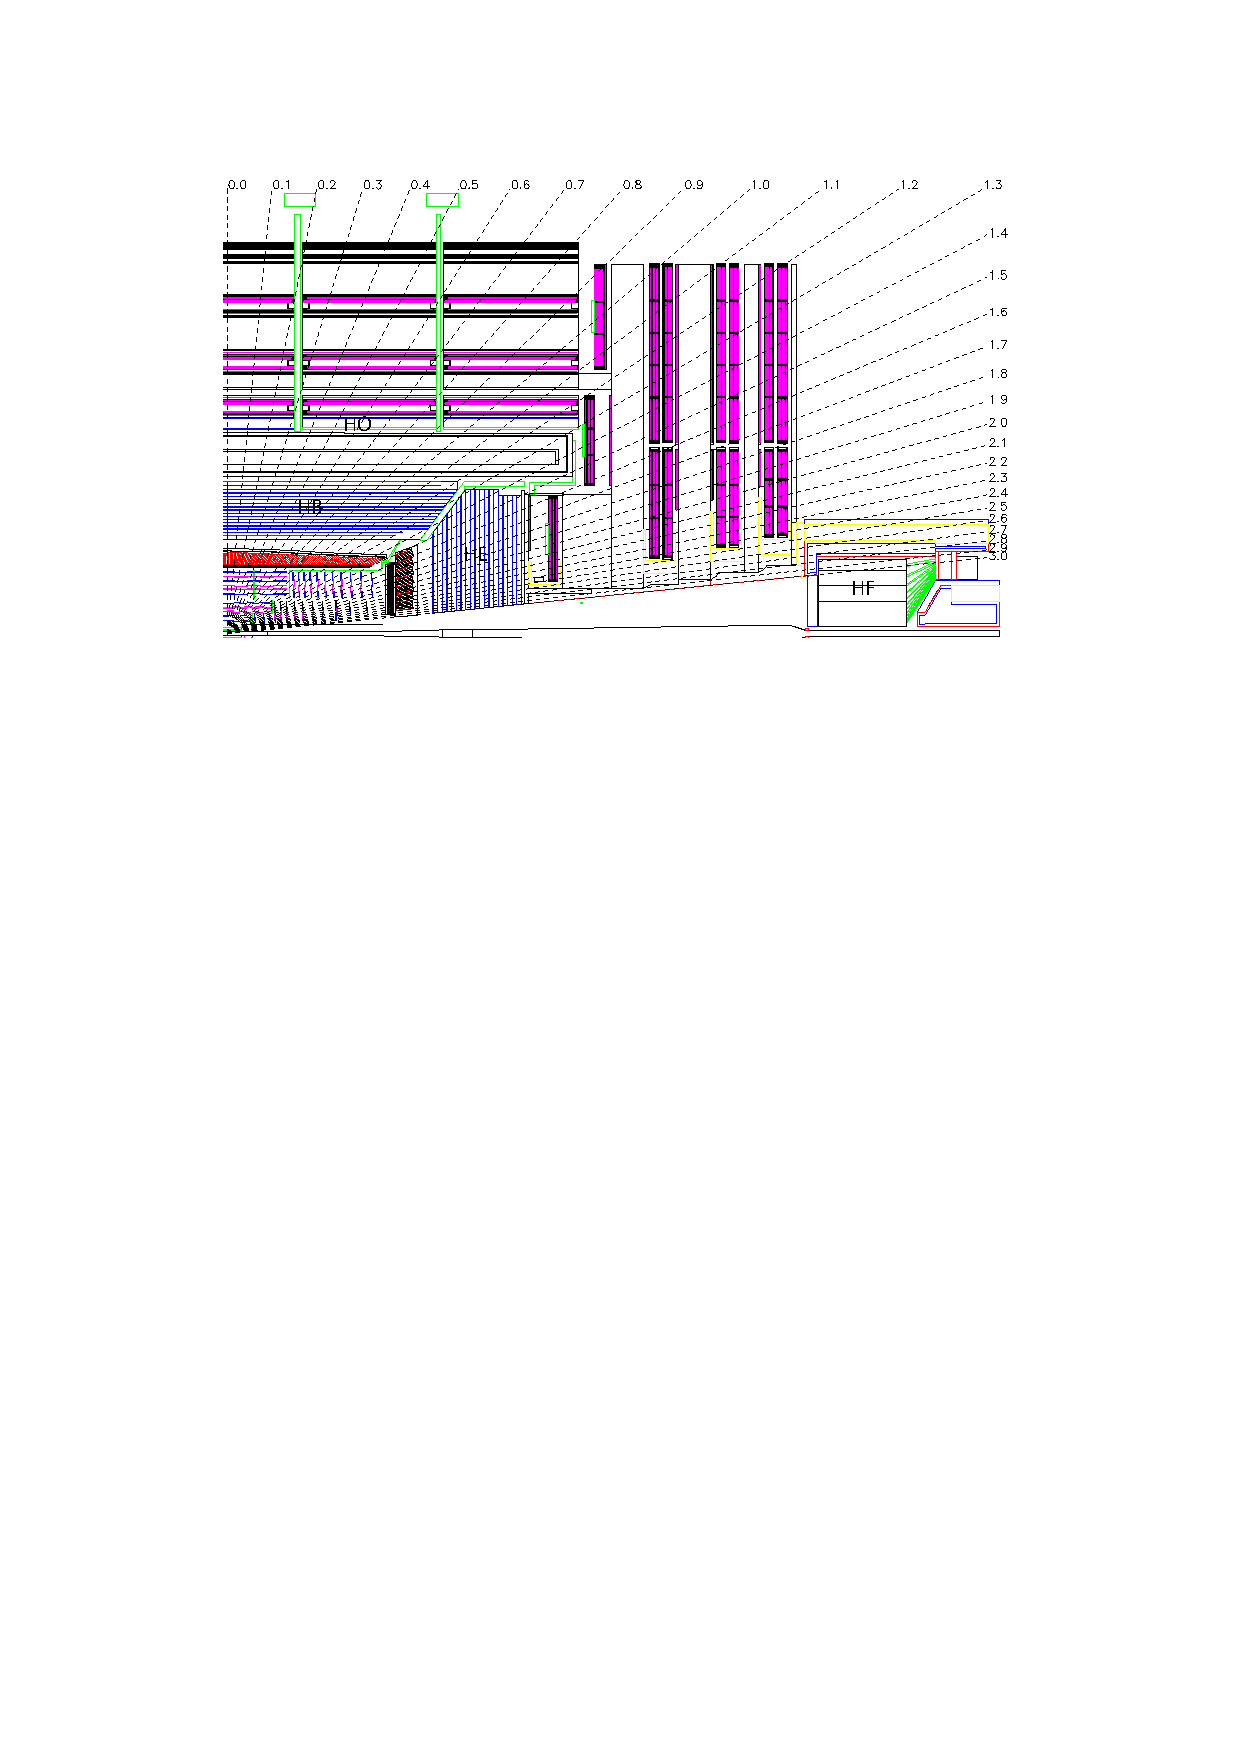
\includegraphics[width=0.9\textwidth]{plots/detector/hcal_layout.pdf}
\caption{Transverse section through the \ac{HCAL}, indicating its geometry \cite{Chatrchyan:2008aa}.}
\label{fig:hcal}
\end{figure}

Both the granularity and the energy resolution of the \ac{HCAL} are worse than
the \ac{ECAL}. The resolution is measured using a test beam of charged pions and
found to be:

\begin{equation}
\frac{\sigma}{E} = \frac{1.2\GeV^{0.5}}{\sqrt{E}} \oplus 0.069,
\end{equation}

where $E$ is the energy of the showering particle. 


\subsection{Muon Detector}
\label{sec:muondetector}

\subsection{Triggering and data processing}
\label{sec:trigger}
